\chapter{深層状態空間モデルの問題点}
\label{chap:baseline}

深層状態空間モデルを用いてより複雑な環境の映像予測を考える場合,潜在的な情報が多くなるはずであるためより大きな状態表現を扱えるようモデルを大きくする必要がある.素朴には状態変数の次元を大きくすることがよいと考えられるが,予備実験の中で深層状態空間モデルは状態変数の次元を大きくすると学習が困難になる,または学習が安定しにくくなることがわかった.まずこのことを示した上で,この理由を考察する.

\begin{figure}[bp]
  \begin{center}
    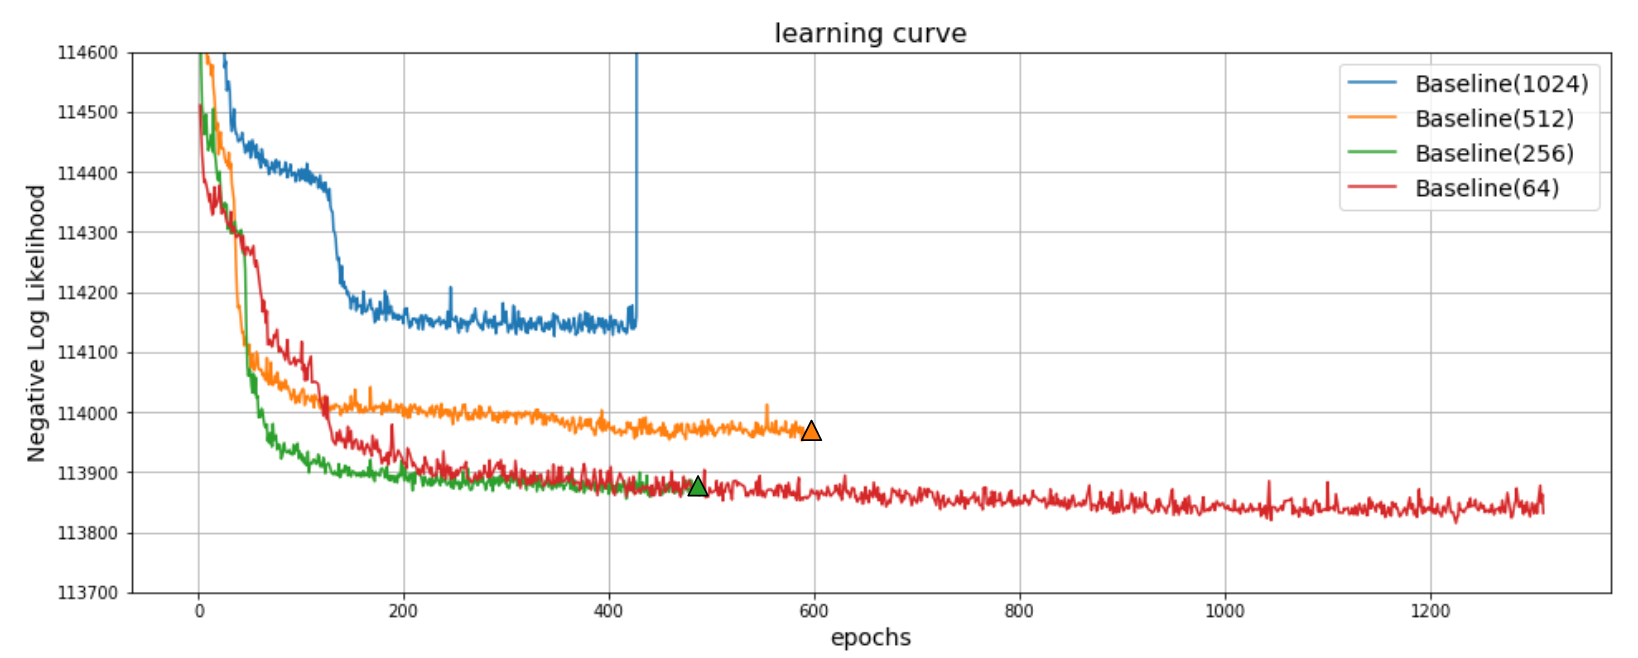
\includegraphics[width=\linewidth]{./figures/dssm_curve.png}
    \caption[状態変数の次元を変えた時のDSSMの学習曲線]{状態変数の次元を変えた時のDSSMの学習曲線.横軸がepoch数で縦軸が目的関数の値である.グラフ中に三角で示されるのは目的関数の値にNaNが出力されてしまったことを示す.Baseline(1024)は400epochを過ぎたあたりで目的関数の値が発散し異常な値をとっている.}
    \label{fig:dssm_curve}
  \end{center}
\end{figure}

\section{学習が失敗した例}
図 \ref{fig:dssm_curve}は,通常のDSSMモデルを状態変数の次元を何通りかに変えてモデルを構築し,学習時の訓練用データでの目的関数の値の増減をプロットしたものである.状態変数を比較的低次元の64次元に設定すると順調に学習が進み,図 \ref{fig:dssm_base}の左図に示すように少しずつ近い映像が出力されるようになる.しかし状態変数の次元を512次元に設定すると明らかに精度が悪化し,1024次元にするとさらに悪化している.図 \ref{fig:dssm_base}の右図は1024次元での実験で目的関数の値が発散した後の生成映像の様子で,他の次元で学習が失敗した場合も同じような映像が生成される.256次元や512次元での実験で途中から目的関数の値にNaNが出力されてしまうのは,第\ref{chap:experiment}章の「実験の安定化」で述べるように,カルバックライブラー距離を小さくすることに失敗しゼロ除算が発生したためである.1024次元で値が発散している理由は定かでないが,256次元,512次元と同様の理由であると考えられる.

\begin{figure}[tp]
  \begin{center}
    \subfloat[][学習が進んでいる例]{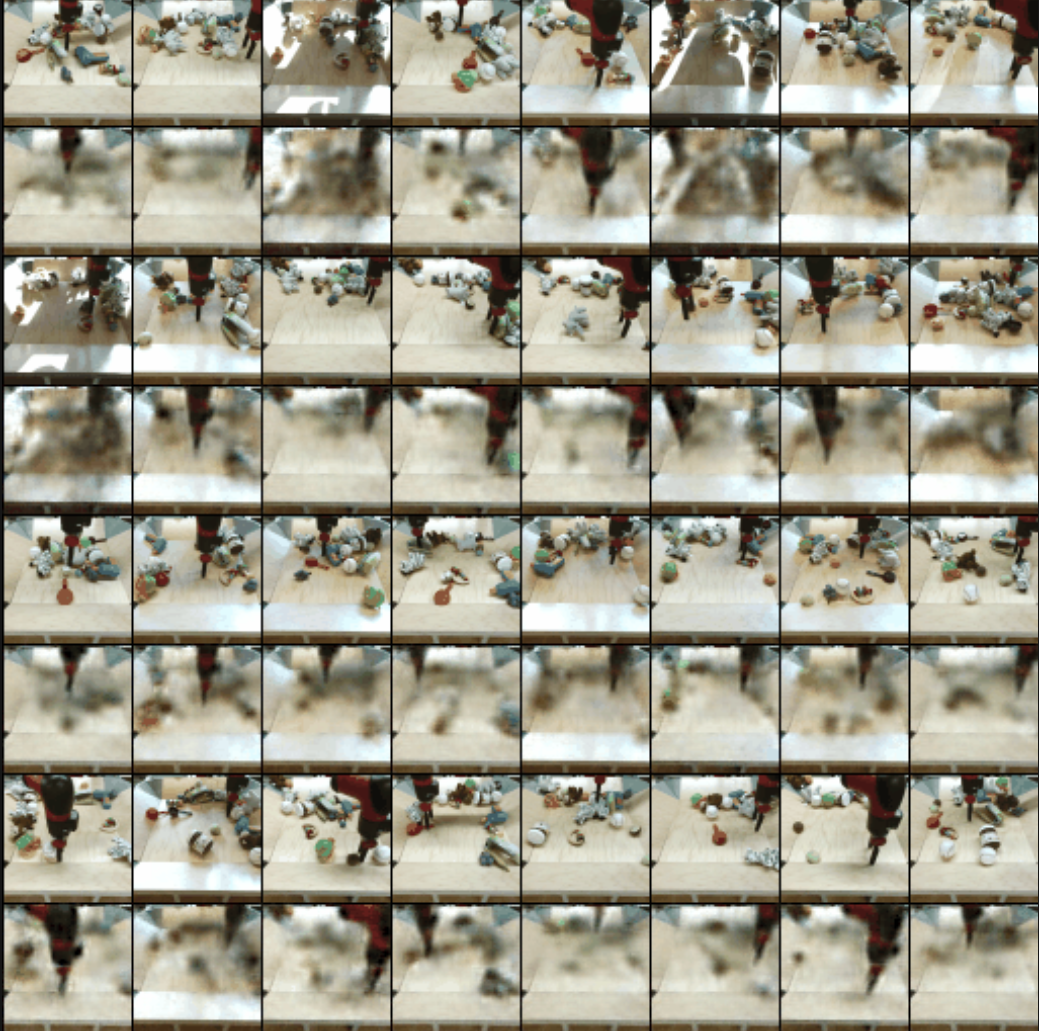
\includegraphics[width=0.46\linewidth]{./figures/dssm_64.png}} \quad
    \subfloat[][学習が失敗した例]{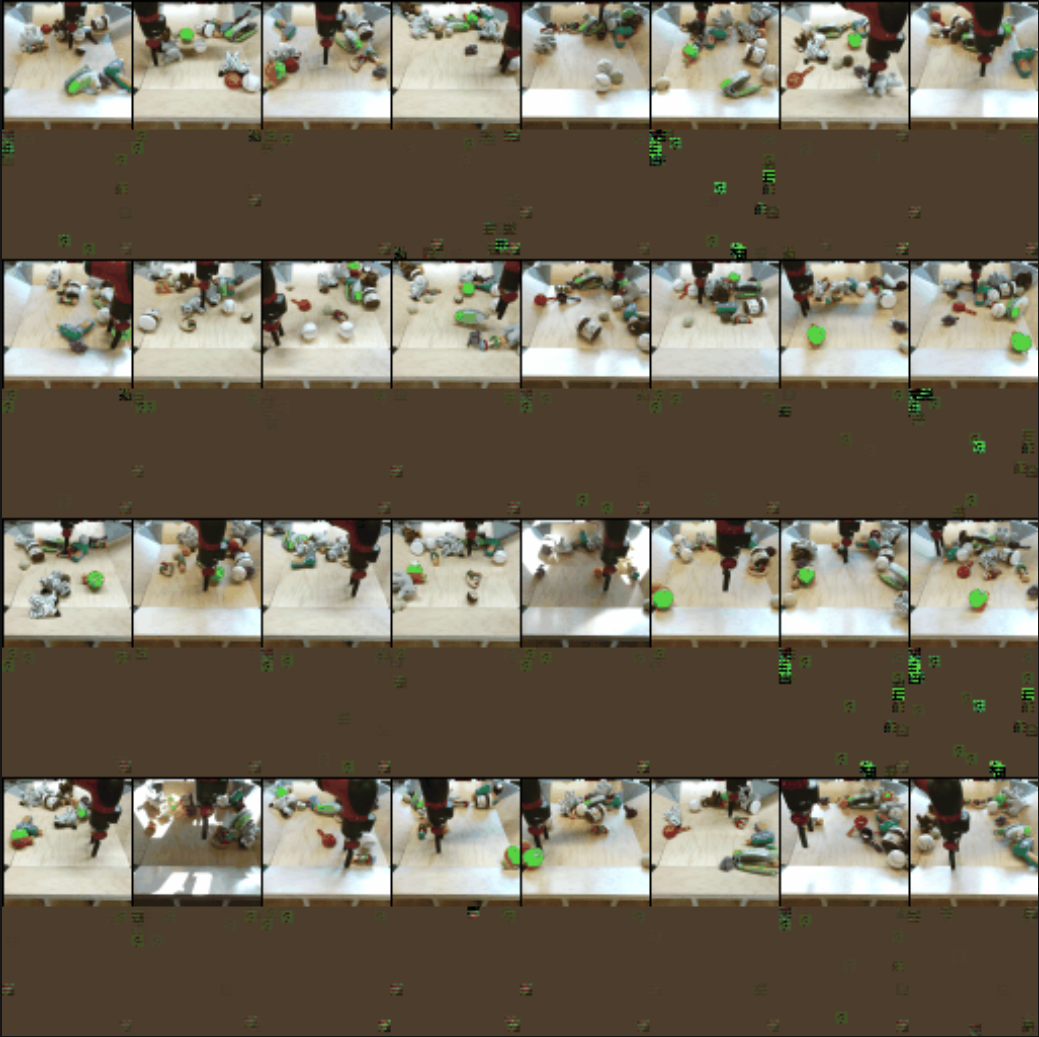
\includegraphics[width=0.46\linewidth]{./figures/dssm_1024.png}}
    \caption[DSSMの学習中にサンプルされた映像の例]{DSSMの学習中にサンプルされた映像の例.上から奇数段目が正解映像で,上から偶数段目が一段上の映像の行動条件付き映像予測結果である.10フレームの映像予測を行っているが,図ではある一時刻の観測のみが示されている}
  \end{center}
  \label{fig:dssm_base}

\end{figure}

ELBOがNaNをとったり発散したりすることは数値計算の丸め誤差などの理由も関わるので一旦考えないとしても,明らかに状態変数の次元を大きくすることで精度が下がっていることが図 \ref{fig:dssm_curve}からわかる.

\section{学習が難しくなる理由の考察}
VAEの学習では前節で述べたような問題は起こらないことを踏まえると,DSSMで学習が難しいのは状態変数の遷移の部分であると考えられる.さらに,状態変数に高次元を仮定したとき,状態変数の遷移の部分では状態変数の生成モデル・推論モデルともに高次元ベクトルから高次元ベクトルへの写像を学習する必要が生じてまずこの部分で学習に時間がかかりやすくなっており,さらに推論モデルが十分に学習されないまま状態変数の事前分布と事後分布のカルバックライブラー距離の最小化が図られてしまうので,学習が安定しにくなっていると考えられる.

このことから,単に状態変数を高次元にすることはDSSMの性質上適切ではなく,DSSMをより複雑な環境を扱う問題にスケールさせるためには他の方法を考える必要がある.以上の予備実験を受け,次章ではシンプルなDSSMの拡張方法を提案する.
